%%
%% Copyright 2007, 2008, 2009 Elsevier Ltd
%%
%% This file is part of the 'Elsarticle Bundle'.
%% ---------------------------------------------
%%
%% It may be distributed under the conditions of the LaTeX Project Public
%% License, either version 1.2 of this license or (at your option) any
%% later version.  The latest version of this license is in
%%    http://www.latex-project.org/lppl.txt
%% and version 1.2 or later is part of all distributions of LaTeX
%% version 1999/12/01 or later.
%%
%% The list of all files belonging to the 'Elsarticle Bundle' is
%% given in the file `manifest.txt'.
%%

%% Template article for Elsevier's document class `elsarticle'
%% with numbered style bibliographic references
%% SP 2008/03/01

\documentclass[preprint,12pt, a4paper]{elsarticle}

%% Use the option review to obtain double line spacing
%% \documentclass[authoryear,preprint,review,12pt]{elsarticle}

%% For including figures, graphicx.sty has been loaded in
%% elsarticle.cls. If you prefer to use the old commands
%% please give \usepackage{epsfig}

%% The amssymb package provides various useful mathematical symbols
\usepackage{amssymb}
%% The amsthm package provides extended theorem environments
%% \usepackage{amsthm}

%% The lineno packages adds line numbers. Start line numbering with
%% \begin{linenumbers}, end it with \end{linenumbers}. Or switch it on
%% for the whole article with \linenumbers.
\usepackage{lineno}

\usepackage{float}
\restylefloat{table}

\usepackage[colorlinks=true, urlcolor=blue, pdfborder={0 0 0}]{hyperref}
\usepackage{breakurl}
\usepackage[htt]{hyphenat}


\journal{SoftwareX}

\begin{document}
\begin{frontmatter}

\title{\texttt{davos}: The Python package smuggler}
\author{Paxton C. Fitzpatrick}
\author{Jeremy R. Manning\corref{cor}}
\ead{Jeremy.R.Manning@Dartmouth.edu}
\cortext[cor]{Corresponding author}
\address{Department of Psychological and Brain Sciences\\Dartmouth College, Hanover, NH 03755}

% ------------------------------------------------------ ABSTRACT ------------------------------------------------------

\begin{abstract}
% 100-word limit (though many published articles don't seem to conform to this?)
% \texttt{davos} is a Python package for creating self-managing, reproducible workflows that specify dependencies directly in their code, and install them
% \texttt{davos} is a Python package that enables creating and sharing reproducible workflows as a single, ready-to-run IPython notebook.

%davos is a python package for creating, sharing, and running reproducible code without the need for

TODO: clean up after writing body

Reproducible code plays many important roles in modern scientific research: it enables scientists to collaborate on projects,\comment{parallelize data collection across multiple sites or machines} replicate and extend prior work, and teach students new concepts and techniques via hands-on, interactive tutorials.
However, existing tools that facilitate creating, sharing, and running reproducible code are often highly complex and resource-intensive, creating barriers to both contributing to and benefitting from open science resources.
Here, we introduce \texttt{davos}, a Python package that allows users to create and share reproducible workflows...


%Many important parts of modern scientific research depend on writing, sharing, and running reproducible code. It enables scientists to collaborate on projects, replicate and extend prior work, and teach students new ideas and techniques through hands-on, interactive tutorials.

%The ability to write, share, and run reproducible code plays many important roles in modern scientific research:

%Writing and sharing reproducible code plays an important role in modern scientific research, enabling scientists to collaborate on projects, replicate and extend previous work, and teach students concepts and techniques through

%\texttt{davos} is a Python package that provides a simple, accessible, and effective way to manage and share reproducible code.

%\texttt{davos} provides the \texttt{smuggle} statement

%\texttt{davos} is a Python package that allows users to write, run, and share reproducible Python code without the need for containers or virtual environments.

%davos is a Python package that allows users to manage and share reproducible code without the need for containers or virtual environments.

%\texttt{davos} is a Python package for creating, running, and sharing reproducible workflows without the need for external containerized or virtualized environments.

%\texttt{davos} is a Python package that makes writing, running, and sharing reproducible code easy. Importing \texttt{davos} in an IPython notebook enables the \textit{smuggle} statement: a drop-in replacement for the built-in \textit{import} statement that can install missing packages as needed at runtime, and may be

%\texttt{davos} is a Python package for creating self-managing, reproducible workflows that specify dependencies directly within their code and install packages as needed at runtime.

%\texttt{davos} works by providing the \textit{smuggle} statement: a drop-in replacement for the built-in \texttt{import} statement that  \_\_\_, and the

\end{abstract}


\begin{keyword}
Reproducibility \sep Open science \sep Python \sep Jupyter Notebook \sep Google Colaboratory \sep Package management
\end{keyword}

\end{frontmatter}


% ------------------------------------------------------ METADATA ------------------------------------------------------
\section*{Required Metadata}

\section*{Current code version}


\begin{table}[H]
\begin{tabular}{|l|p{6.5cm}|p{6.5cm}|}
\hline
\textbf{Nr.} & \textbf{Code metadata description} & \textbf{Please fill in this column} \\
\hline
C1 & Current code version &  v0.1.1 \\
\hline
C2 & Permanent link to code/repository used for this code version & \url{https://github.com/ContextLab/davos/tree/v0.1.1} \\
\hline
C3 & Code Ocean compute capsule & \\
\hline
C4 & Legal Code License & MIT \\
\hline
C5 & Code versioning system used & git \\
\hline
C6 & Software code languages, tools, and services used & Python, JavaScript, PyPI/pip, IPython, Jupyter, Ipykernel, PyZMQ. Additional tools used for tests: pytest, Selenium, Requests, mypy, GitHub Actions \\
\hline
C7 & Compilation requirements, operating environments \& dependencies & Dependencies:~Python$>$=3.6, packaging, setuptools.~Supported OSes: MacOS, Linux, Unix-like.~Supported IPython environments: Jupyter notebooks, JupyterLab, Google Colaboratory, Binder, IDE-based notebook editors. \\
\hline
C8 & If available Link to developer documentation/manual & \url{https://github.com/ContextLab/davos\#readme} \\
\hline
C9 & Support email for questions & contextualdynamics@gmail.com \\
\hline
\end{tabular}
\caption{Code metadata}
\label{}
\end{table}

\linenumbers


% --------------------------------------------- MOTIVATION & SIGNIFICANCE ----------------------------------------------
\section{Motivation and significance}
Modern scientific research frequently entails writing software code for a wide variety of purposes throughout the scientific process.
Researchers across disciplines may design and implement complex experiments; collect, store, and analyze large datasets; create visualizations for presentations and publications; and share their findings and techniques with peers, students, and the broader public through tutorials, demos, workshops, and classes.
However, one fundamental requirement of virtually any form of research-related code is that its behavior and outputs remain consistent and predictable, no matter when, where, or by whom it is run.
This stability can be crucial, for example, to ensuring that data are collected under the same conditions (e.g., across recordings, subjects, or physical locations)
%^ or locations, e.g., in different test rooms, on different machines, at different sites, etc.
over multiple months or years, and that they can be accessed, processed, and analyzed consistently by a research team that may be spread across multiple institutions or countries.
Additionally, modern open science practices encourage publicly sharing research code and data so that others may explore, reproduce, learn from, and build upon existing work.
Much of the benefit afforded by freely available research code depends on users' ability to execute it and achieve the same result as its original author.

Python \cite{vanR95} has become one of the most widely used and fastest-growing scientific programming languages, in part by combining an accessible, high-level syntax with a rich ecosystem of powerful third-party tools that facilitate rapid development and collaboration \cite{MullEtal15}.
The Python ecosystem offers an extensive data science toolkit with platforms for interactive programming (e.g., Project Jupyter \cite{KluyEtal16}, Google Colaboratory), community-maintained libraries for data manipulation (e.g., NumPy \cite{HarrEtal20}, SciPy \cite{VirtEtal20}, Pandas \cite{McKi10}) and visualization (e.g., Matplotlib \cite{Hunt07}, seaborn \cite{Wask21}), frameworks for training complex machine learning models (e.g., scikit-learn \cite{PedrEtal11}, TensorFlow \cite{AbadEtal15}, Hugging Face \cite{WolfEtal20}), and myriad other resources.
However, this heavy emphasis on third-party libraries also presents a challenge to writing and sharing stable, reproducible scientific Python code:
different versions of the same library may behave differently, adopt changes in syntax, expose different functions and interfaces, add or drop support for specific hardware or software, write (or expect to read) files in different formats, fix (or introduce) bugs, and so on.
While these issues exist to some extent in any software language or ecosystem, they have a particular impact on the Python community due to its unusually rapid growth relative to other languages.
Ensuring Python code behaves consistently over time and across users therefore typically requires ensuring it is always run with the same specific set of versions for each third-party package used.
%Ensuring Python code behaves consistently over time and across users therefore typically requires guaranteeing that the same specific version of each required third-party package is used, every time it is run.

One common approach to solving this problem is to create containerized or virtualized Python environments (e.g., using Docker \cite{Merk14}, Singularity \cite{KurtEtal17}, or conda \cite{Anac12}) tailored to individual applications.
A researcher may build such an environment around a particular experiment or analysis pipeline, and exclusively run their code from inside it, ``entering" and ``exiting" the environment before and after each time they do so.
They can also distribute their custom environment alongside their code as a configuration file that explicitly lists required package versions, enabling others to build identical copies for themselves.
This allows research teams to deploy experiments on multiple machines for more efficient data collection, collaborate on analyses without introducing conflicts or inconsistencies, and publicly share their study designs and results for others to reproduce, replicate, or adapt to study new questions in the future.

While often effective, this approach bears two notable drawbacks.
First, it can add substantially to the technical knowledge, computing resources, and initial setup needed to run or share the actual code of interest.
For example, sharing code for an analysis or tutorial that relies on a particular Docker image to run properly would of course necessitate writing and distributing extra configuration files and setup instructions.
But far more burdensomely, it also requires that anyone who may want to run the code (in addition to the author seeking to share it!) first be able to install and navigate additional software that is likely far more complex and resource-intensive than the actual analysis or tutorial code it facilitates running.
This can introduce a need for both a degree of computer literacy and computational resources that may not be universally accessible, particularly to students or other early-career scientists hoping to learn from publicly available tutorials.
These added prerequisites clash with the simplicity and accessibility that have contributed to Python's popularity, and can create significant barriers to both contributing to and taking advantage of open science resources.

Second, while many existing tools allow users to initially populate a Python environment with a fixed set of packages and package versions (e.g., from a \texttt{requirements.txt}, \texttt{pyproject.toml}, \texttt{environment.yml}, \texttt{Pipfile}, \texttt{Dockerfile RUN} instruction, etc.), few, if any, ensure that these specified requirements \textit{remain} satisfied after they are first installed.
The ability to modify an environment after its creation is useful in many cases (e.g., to install additional software, when needed). However, this also makes it easy to inadvertently alter existing packages, potentially leading to subtle issues with code that relies on them.
For instance, suppose a researcher has implemented a series of analyses using version 1.0 of ``Package \textit{X}," and decides to  perform an additional analysis that requires installing ``Package \textit{Y}."
If Package \textit{Y} depends on version 0.9 of Package \textit{X}, then Package \textit{X} will be downgraded to accommodate this new requirement, potentially altering or breaking prior analyses for both the researcher and anyone with whom their code may be shared.
Further, if certain analyses require Package \textit{Y} while others rely on a feature of Package \textit{X} not implemented until version 1.0, it's unclear which version the researcher should install in the environment.



%Introduce the scientific background and the motivation for developing the software.

%Explain why the software is important, and describe the exact (scientific) problem(s) it solves.

%Indicate in what way the software has contributed (or how it will contribute in the future) to the process of scientific discovery; if available, this is to be supported by citing a research paper using the software.

%Provide a description of the experimental setting (how does the user use the software?).

%Introduce related work in literature (cite or list algorithms used, other software etc.).


% ------------------------------------------------ SOFTWARE DESCRIPTION ------------------------------------------------
\section{Software description}
% Describe the software in as much as is necessary to establish a vocabulary needed to explain its impact.


\subsection{Software Architecture}
% Give a short overview of the overall software architecture; provide a pictorial component overview or similar (if possible). If necessary provide implementation details.


\subsection{Software functionalities}%\label{sec:functionalities}

\subsubsection{The \texttt{smuggle} statement}
Importing \texttt{davos}\comment{in a Jupyter notebook} enables an additional Python keyword: ``\texttt{smuggle}".
The \texttt{smuggle} statement can be used as a drop-in replacement for Python's built-in \texttt{import} statement to load libraries, modules, and other objects into the current namespace.
However, whereas \texttt{import} will fail if the requested package is not installed locally, \texttt{smuggle} statements can handle missing packages on the fly.
If a smuggled package does not exist in the local environment, \texttt{davos} will install it, expose its contents to Python's \texttt{import} machinery, and load it into the namespace for immediate use.


\subsubsection{The onion comment}
For greater control over the behavior of \texttt{smuggle} statements, \texttt{davos} defines an additional construct called the \textit{onion comment}. An onion comment is a special type of inline comment that may be placed on a line containing a \texttt{smuggle} statement to customize how \texttt{davos} searches for the smuggled package locally and, if necessary, how it should be installed. Onion comments follow a simple syntax based on the ``type comment" syntax introduced in PEP 484 \cite{vanREtal14} and are designed to make managing packages via \texttt{davos} intuitive and familiar. To construct an onion comment, simply provide the name of the installer program (e.g., \texttt{pip}) and the same arguments one would use to install the package as desired manually via the command line (see Fig.~\ref{fig:snippet1}).

\begin{figure}[h]
\centering
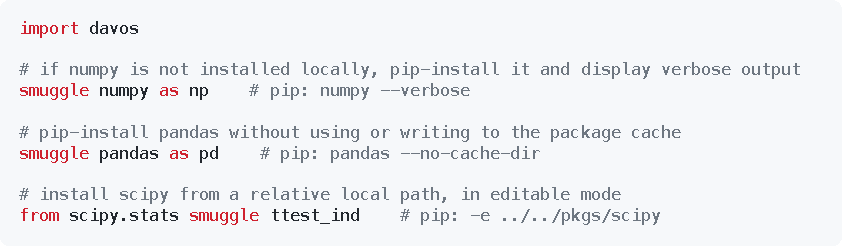
\includegraphics[width=\textwidth]{snippets/snippet1.pdf}
\caption{\small \textbf{Figure 1}}
\label{fig:snippet1}
\end{figure}



%\definecolor{backgroundgrey}{RGB}{244,246,249}
%\definecolor{commentgrey}{RGB}{91,99,110}
%\definecolor{keywordred}{RGB}{194,11,36}
%
%\lstset{
%    backgroundcolor=\color{backgroundgrey},
%    basicstyle=\footnotesize\fontfamily{qag}\selectfont, %\ttfamily,
%    breaklines=true,
%    commentstyle=\color{commentgrey},
%    language=Python,
%    emph={import, smuggle, from, as},
%    emphstyle=\color{keywordred},
%}
%
%\begin{lstlisting}
%import davos
%
%# if numpy is not installed locally, pip-install it and display verbose output
%smuggle numpy as np    # pip: numpy --verbose
%
%# pip-install pandas without using or writing to the package cache
%smuggle pandas as pd    # pip: pandas --no-cache-dir
%
%# install scipy from a relative local path, in editable mode
%from scipy.stats smuggle ttest_ind # pip: -e ../../pkgs/scipy
%\end{lstlisting}

\subsubsection{The \texttt{davos} config}

\subsubsection{Additional functionality}

% Present the major functionalities of the software.


\subsection{Sample code snippets analysis (optional)}


% ----------------------------------------------- ILLUSTRATIVE EXAMPLES ------------------------------------------------
\section{Illustrative Examples}
% Provide at least one illustrative example to demonstrate the major functions.

% Optional: you may include one explanatory video that will appear next to your article, in the right hand side panel. (Please upload any video as a single supplementary file with your article. Only one MP4 formatted, with 50MB maximum size, video is possible per article. Recommended video dimensions are 640 x 480 at a maximum of 30 frames/second. Prior to submission please test and validate your .mp4 file at $ http://elsevier-apps.sciverse.com/GadgetVideoPodcastPlayerWeb/verification$. This tool will display your video exactly in the same way as it will appear on ScienceDirect.).


% ------------------------------------------------------- IMPACT -------------------------------------------------------
\section{Impact}
\comment{
- research domain-independent application
- applicability not limited to research
  - regression (?) testing
- mention something about not having to teach environment management to teach day 1 python lesson, or spend hours debugging conda installation in order to share tutorial or demo with students
}

Despite the short time since its conception and initial release, \texttt{davos} has already found use in a variety of applications.
In addition to managing data analysis environments for multiple ongoing research studies, \texttt{davos} is being used by both students and instructors in programming courses such as \href{https://github.com/ContextLab/storytelling-with-data}{\textit{Storytelling with Data}} \cite{Mann21b} (an open course on data science, visualization, and communication) to simplify distributing lessons and submitting assignments, as well as in online demos such as {\texttt{abstract2paper}} \cite{Mann21a} (an example application of \href{https://github.com/EleutherAI/gpt-neo}{GPT-Neo}) to share ready-to-run code that installs dependencies automatically.

%\textbf{This is the main section of the article and the reviewers weight the description here appropriately}

%Indicate in what way new research questions can be pursued as a result of the software (if any).

%Indicate in what way, and to what extent, the pursuit of existing research questions is improved (if so).

%Indicate in what way the software has changed the daily practice of its users (if so).

%Indicate how widespread the use of the software is within and outside the intended user group.

%Indicate in what way the software is used in commercial settings and/or how it led to the creation of spin-off companies (if so).


% ---------------------------------------------------- CONCLUSIONS -----------------------------------------------------
\section{Conclusions}
% Set out the conclusion of this original software publication.


\section*{Author Contributions}
\textbf{Paxton C. Fitzpatrick}: Conceptualization, Methodology, Software, Validation, Writing - Original Draft, Visualization. \textbf{Jeremy R. Manning}: Conceptualization, Resources, Writing - Review \& Editing, Supervision, Funding acquisition.

\section*{Funding}
Our work was supported in part by NSF grant number 2145172 to J.R.M.
The content is solely the responsibility of the authors and does not necessarily represent the official views of our supporting organizations.


\section*{Declaration of Competing Interest}
We wish to confirm that there are no known conflicts of interest associated with this publication and there has been no significant financial support for this work that could have influenced its outcome.


\section*{Acknowledgements}


%---------------------------------------------------- BIBLIOGRAPHY -----------------------------------------------------
\bibliographystyle{elsarticle-num}
\bibliography{main.bib}

\end{document}

